\documentclass[sigconf,authorversion,nonacm]{acmart}

\settopmatter{printacmref=false}

\usepackage{amsmath}
\usepackage{algorithm}
\usepackage{algpseudocode}
\usepackage{booktabs}
\usepackage{enumitem}
\usepackage{float}
\usepackage{makecell}
\usepackage{xcolor}

\definecolor{attncolor}{RGB}{30,100,200}   % blue-ish
\definecolor{mlpcolor}{RGB}{200,80,30}     % orange-ish
\newcommand{\todoadd}[1]{%
  \par\noindent
  \begingroup
  \setlength{\fboxsep}{4pt}%
  \colorbox{yellow!35}{\parbox{\dimexpr\linewidth-2\fboxsep\relax}{\textbf{TODO add this:} #1}}%
  \endgroup
  \par
}

% Bold the full reference while keeping the entire phrase clickable.
\newcommand{\strongtabref}[1]{\hyperref[#1]{\textbf{Table~\ref*{#1}}}}
\newcommand{\strongfigref}[1]{\hyperref[#1]{\textbf{Figure~\ref*{#1}}}}
\newcommand{\strongalgref}[1]{\hyperref[#1]{\textbf{Algorithm~\ref*{#1}}}}
\newcommand{\strongappref}[1]{\hyperref[#1]{\textbf{Appendix~\ref*{#1}}}}
\newcommand{\strongsecref}[1]{\hyperref[#1]{\textbf{Section~\ref*{#1}}}}

\graphicspath{{figures/}}

%%
%% \BibTeX command to typeset BibTeX logo in the docs
\AtBeginDocument{%
  \providecommand\BibTeX{{%
    Bib\TeX}}}

\begin{document}

\title{Parallelizing GPT-2 --- ``It works on my GPU''}

\author{Jack ``Siggy'' Sigler}
\affiliation{%
 \institution{Colorado School of Mines}
 \city{Golden}
 \state{CO}
 \country{USA}
 }

\author{Sam Abderholden}
\affiliation{%
 \institution{Colorado School of Mines}
 \city{Golden}
 \state{CO}
 \country{USA}
}

\author{Dawson Matthews}
\affiliation{%
 \institution{Colorado School of Mines}
 \city{Golden}
 \state{CO}
 \country{USA}
}

\maketitle

\section{Introduction of the Paper and the Targeted Problem}

\todoadd{Introduce the targeted problem, motivate why accelerating the forward pass of a GPT-style model matters, summarize the serial-to-CUDA progression used in this project, and briefly preview the main performance results and contributions.}

\section{Serial Implementation and Analysis}

\subsection*{Problem Background}

In this project, we implement an optimized CUDA version of the forward pass of Andrej Karpathy's \textit{microgpt} \cite{karpathyMicrogpt2026}. \textit{Microgpt} is a minimal, dependency-free Python implementation of a GPT-style model. It is based on the GPT-2 architecture \cite{radfordLanguageModelsAre2019}, with a few changes made for simplicity. Both GPT-2 and Karpathy's \textit{microgpt} implement:
\begin{itemize}[noitemsep, topsep=0pt]
  \item Decoder-only Transformer architecture
  \item Token + positional embeddings
  \item Stacked Transformer blocks
  \item Causal (masked) multi-head self-attention
  \item Residual connections around attention and MLP sublayers
  \item Feedforward MLP with expansion and projection
  \item Autoregressive next-token prediction
\end{itemize}
Since \textit{microgpt} was intended to showcase the GPT-2 architecture in a single unoptimized Python file, the proposed model has only 4,192 parameters compared to GPT-2's 1.6 billion parameters. In addition to the reduced model size, \textit{microgpt} introduces several simplifications, including the use of RMSNorm instead of LayerNorm, removal of bias terms, and ReLU in place of GELU \cite{karpathyMicrogpt2026}. 

\noindent In order to keep the scope of our implementation to 10 hours, we focus only on speeding up the forward pass of \textit{microgpt}. Since we believed that comparing a CUDA C++ version to a Python version would introduce speedups due to both our parallelization choices and language differences (C++ vs Python), we first reimplemented \textit{microgpt} in C++, preserving the following:
\begin{itemize}[noitemsep, topsep=0pt]  \item Identical layer structure
  \item Same ordering of operations (norm $\rightarrow$ attention $\rightarrow$ residual $\rightarrow$ norm $\rightarrow$ MLP $\rightarrow$ residual)
  \item Same KV caching mechanism
  \item Same attention computation (scaled dot-product + softmax)
  \item Same MLP structure (\texttt{fc1} $\rightarrow$ activation $\rightarrow$ \texttt{fc2})
\end{itemize}

Our C++ version is nearly identical, with differences limited to implementation details such as replacing dynamic Python data structures with pre-allocated caches, removing autograd in favor of raw floating-point computation, and expressing all operations as explicit loop-based computations over contiguous memory.

\subsection*{C++ Serial Baseline}
Our implementation follows the training setup used in \textit{microgpt}, which operates on a character-level dataset consisting of a set of names $\mathcal{D} = \{s^{(1)}, s^{(2)}, \dots, s^{(N)}\}$. Each name $s^{(k)} \in \mathcal{D}$ is treated as a sequence of tokens, $s^{(k)} = [t_1, t_2, \dots, t_T]$, where $T$ denotes the sequence length. The model is trained autoregressively to predict the next token given all previous tokens. Our C++ implementation preserves this setup exactly, performing the same forward-pass computation and next-token prediction task. The prompt used to generate the 
C++ baseline can be found under \strongappref{appendix:serial-prompt}
 
Given a tokenized sequence (i.e., a single name) $[t_1, t_2, \dots, t_T]$, the model computes a sequence of logits $[y_1, y_2, \dots, y_{T-1}]$, where each $y_i$ represents the model's prediction of token $t_{i+1}$ conditioned on the prefix $[t_1, \dots, t_i]$. In the baseline implementation, this computation is performed sequentially, iterating over the dataset one name at a time and, within each name, one token at a time, with each position attending over all previous tokens in the sequence.  A high level pseudocode of our serial implentation is shown under \strongalgref{alg:forward-pass}.

We denote the embedding dimension as $d$, the number of Transformer layers as $L$, and the number of attention heads as $H$. For each token position $i$, the model produces a hidden representation $x_i \in \mathbb{R}^d$, which is transformed through attention and MLP operations across all layers. 

The computational cost of the forward pass over $N$ sequences is $O\!\left(N \cdot L \cdot (C_{\text{attn}} + C_{\text{mlp}})\right)$, where $C_{\text{attn}} = O(T^2 \cdot d)$ and $C_{\text{mlp}} = O(T \cdot d^2)$. Since the names have approximately constant sequence lengths, we can simplify this to $O(N \cdot L \cdot d^2)$. 


\begin{algorithm}[H]
\caption{High-Level Forward Pass}
\label{alg:forward-pass}
\begin{algorithmic}
\State $\text{loss} \gets 0$
\For{each sequence $s^{(k)} \in \mathcal{D}$}
    \For{$i = 1$ to $T-1$}
        \State $x_i \gets \text{TokenEmbedding}(t_i) + \text{PositionalEmbedding}(i)$
        \State $x_i \gets \text{RMSNorm}(x_i)$

        \For{$\ell = 1$ to $L$}
            \State $x_i \gets x_i + \text{Attention}(\text{RMSNorm}(x_i), \{k_j, v_j\}_{j \le i})$
            \State $x_i \gets x_i + \text{MLP}(\text{RMSNorm}(x_i))$
        \EndFor

        \State $y_i \gets \text{Linear}(x_i)$
        \State $\text{loss} \gets \text{loss} - \log(\text{Softmax}(y_i)[t_{i+1}])$
    \EndFor
\EndFor
\State $\text{loss} \gets \text{loss} / \text{total\_tokens}$
\end{algorithmic}
\end{algorithm}

Using the \textit{perf time} command we were able to get high level timing characteristics of the C++ baseline program, especially how much time our C++ baseline was performing OS overhead versus useful compute work. With nearly zero system time (0.008s out of 2.74s total) and only 269 context switches, the program runs almost entirely in userspace with negligible OS overhead. An IPC of 3.06 with 0.999 CPUs utilized confirms the single core is saturated with compute for the full duration. Next, we used \textit{perf record} in order to perform a call stack analysis of where the program was spending its CPU time. 
We found that \textbf{99.4\%} of runtime is spent in linear matrix multiplications, with \textbf{70.1\%} occurring in the MLP and \textbf{28.3\%} in attention (note the program spends around 0.4\% performing rmnsnorm, Softmax, and embedding operations). While attention is often considered the bottleneck in Transformer models, this aligns with our earlier complexity analysis, as the approximately constant sequence length causes the $d^2$ term to dominate, making the MLP the primary contributor to runtime.
Treating the matrix multiplications together with the remaining targeted primitives as parallelizable gives $p \approx 0.998$, so Amdahl's Law places the theoretical end-to-end speedup ceiling at $\frac{1}{1-p} \approx 500\times$. If the serial baseline runs for longer, closer to an hour, we expect that the parallelizable region could increase beyond $99.8\%$, leading to even larger speedups.

\input{sections/03_parallel_implementation}
\section{Evaluation Strategy}

In this section, we compare a serial C++ baseline, unbatched and batched PyTorch baselines, and our custom parallel CUDA implementation to analyze forward-pass runtime across configurations. We evaluate these methods under three scaling regimes: (i) fixed model size with increasing number of names processed, (ii) fixed number of names with increasing model size, and (iii) scaling both simultaneously.

We do not directly compare performance between our CUDA implementation and \textit{microgpt}, as the pure Python implementation is prohibitively slow (our CUDA implementation is over 10{,}000$\times$ faster on a medium benchmark). However, we use \textit{microgpt} to validate correctness by comparing logits from a single-sequence forward pass against those produced by the original implementation. 

For analyzing results, we will abbreviate methods as UT = unbatched\_torch, BT = batched\_torch, SC = serial\_cpp, and PC = parallel\_cpp. We abbreviate presets as S, M, L, VL, and XL for the standard size sweep, and MS5, MM5, ML5, MVL5, and MXL5 for the 5k-step model sweep.


\section{Performance Analysis}

\subsection{Performance Analysis}
We begin by examining the case of a fixed model size with increasing input name counts, shown in \strongfigref{result:1} below. 

Our PC method outperforms all other baselines across every input size benchmarked. For both SC and UT, this result is unsurprising, as PC is more heavily optimized for this specific workload. More notably, PC also outperforms BT, which is a highly optimized and widely used ML framework. This advantage can largely be attributed to Python overhead in BT, including costs associated with object management and data movement between Python and underlying implementations.

However, a closer examination of the results shows that, while PC currently outperforms BT, its runtime increases more rapidly with input size, whereas BT exhibits near-ideal scaling behavior. It is therefore reasonable to expect that as input sizes continue to grow, particularly to those typical of modern ML workloads, PC will eventually lose its performance advantage.

\begin{figure}[h]
    \centering
    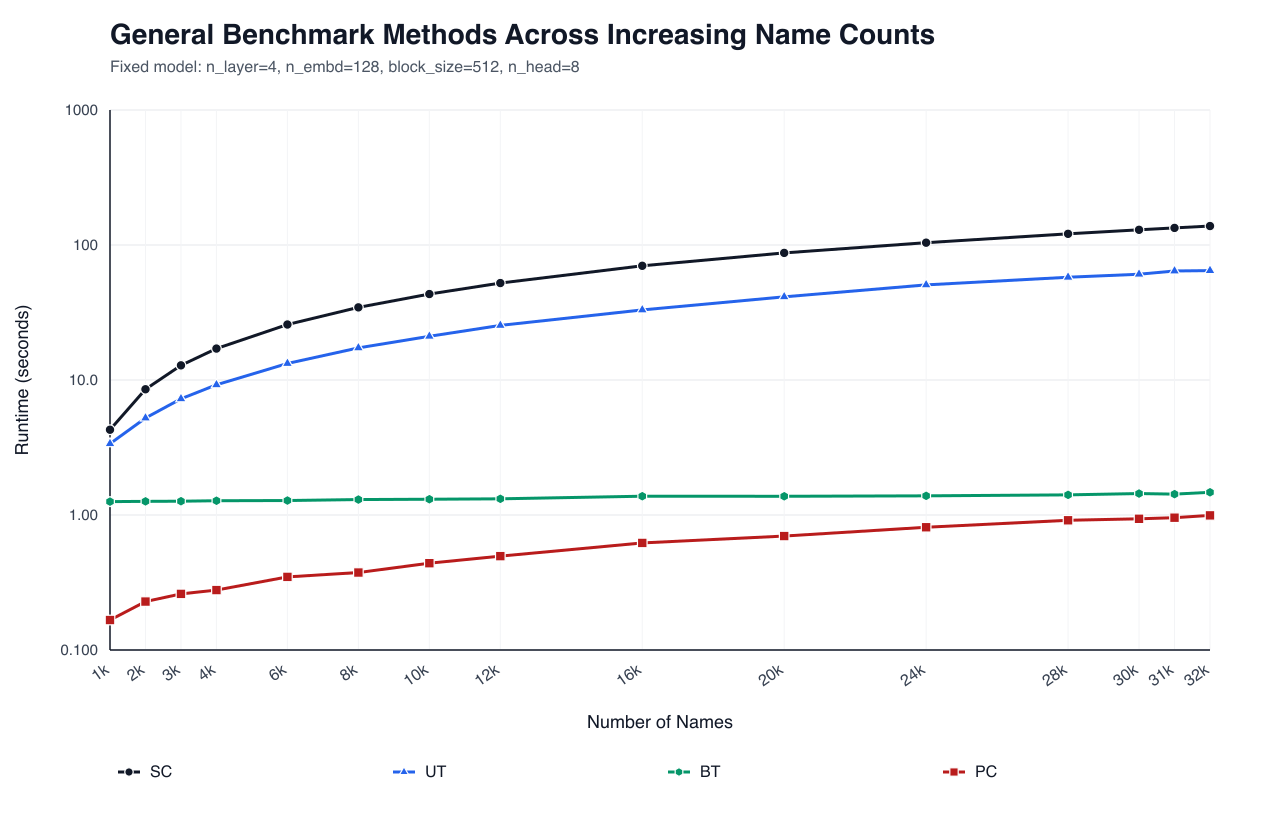
\includegraphics[width=\linewidth]{figures/general_benchmark_names.png}
    \caption{Results from Input Scaling}
    \label{result:1}
\end{figure}


Next we will look at the results from the other two scaling regimes: holding input size constant while increasing model size (ii), and increasing both input size and model size together (iii). The preset definitions for these experiments cam be found in \strongappref{appendix:presets} and the results are shown in \strongtabref{tab:model_configs}.




\begin{table*}[t]
\centering
\small
\begin{minipage}{0.49\textwidth}
\centering
\begin{tabular}{l c c c c}
\toprule
\textbf{Preset} & \textbf{UT} & \textbf{BT} & \textbf{SC} & \textbf{PC} \\
\midrule

MS5 & \makecell{4.33 \\ $0.28\times$}
    & \makecell{0.92 \\ $1.34\times$}
    & \makecell{1.23 \\ $1.00\times$}
    & \makecell{0.20 \\ $6.22\times$} \\

MM5 & \makecell{6.81 \\ $1.58\times$}
    & \makecell{1.10 \\ $9.80\times$}
    & \makecell{10.76 \\ $1.00\times$}
    & \makecell{0.26 \\ $41.38\times$} \\

ML5 & \makecell{12.45 \\ $7.51\times$}
    & \makecell{2.37 \\ $39.45\times$}
    & \makecell{93.53 \\ $1.00\times$}
    & \makecell{0.50 \\ $185.50\times$} \\

MVL5 & \makecell{20.20 \\ $16.21\times$}
     & \makecell{5.79 \\ $56.50\times$}
     & \makecell{327.28 \\ $1.00\times$}
     & \makecell{1.07 \\ $307.03\times$} \\

MXL5 & \makecell{32.29 \\ $24.30\times$}
     & \makecell{12.34 \\ $63.59\times$}
     & \makecell{784.64 \\ $1.00\times$}
     & \makecell{2.10 \\ $373.60\times$} \\


\bottomrule
\end{tabular}
\end{minipage}
\hspace{0.001\textwidth}  % adjust this
\begin{minipage}{0.48\textwidth}
\centering
\begin{tabular}{l c c c c}
\toprule
\textbf{Preset} & \textbf{UT} & \textbf{BT} & \textbf{SC} & \textbf{PC} \\
\midrule


S  & \makecell{2.30 \\ $0.22\times$}
   & \makecell{0.93 \\ $0.54\times$}
   & \makecell{0.50 \\ $1.00\times$}
   & \makecell{0.14 \\ $3.50\times$} \\

M  & \makecell{6.66 \\ $1.62\times$}
   & \makecell{1.07 \\ $10.04\times$}
   & \makecell{10.76 \\ $1.00\times$}
   & \makecell{0.25 \\ $42.40\times$} \\

L  & \makecell{23.32 \\ $8.14\times$}
   & \makecell{2.41 \\ $78.82\times$}
   & \makecell{189.75 \\ $1.00\times$}
   & \makecell{0.76 \\ $250.21\times$} \\

VL & \makecell{64.90 \\ $20.68\times$}
   & \makecell{6.14 \\ $218.60\times$}
   & \makecell{1342.22 \\ $1.00\times$}
   & \makecell{3.06 \\ $438.44\times$} \\

XL & \makecell{127.71 \\ $37.37\times$}
   & \makecell{13.46 \\ $354.55\times$}
   & \makecell{4771.83 \\ $1.00\times$}
   & \makecell{9.18 \\ $519.91\times$} \\

\bottomrule
\end{tabular}
\end{minipage}

\caption{Runtime (top)/speedup (bottom) per method. \textbf{Runtime is in seconds; Speedup is relative to SC}}
\label{tab:model_configs}
\end{table*}

Across both regimes, PC consistently outperforms all baselines, maintaining the largest speedup across almost every preset. This trend holds even as model size increases, demonstrating that the implementation effectively exploits parallelism in the dominant compute paths.

To better interpret these results, we define the forward-pass complexity as $O\bigl(N \cdot L \cdot (C_{\text{attn}} + C_{\text{mlp}})\bigr)$, where $C_{\text{attn}} = T^{2} \cdot d$ and $C_{\text{mlp}} = T \cdot E^{2}$. 
Under the assumption that $T$ remains approximately constant, this simplifies to $\approx O(N \cdot L \cdot d^{2})$.

The empirical trends in \strongtabref{tab:model_configs} align with this analysis. In regime (ii), where $N$ is fixed and model size increases, runtime grows rapidly with $d$ and $L$, consistent with the $d^{2}$ dependence. In regime (iii), where $N$, $L$, and $d$ all increase, the combined effect leads to the largest runtimes, reflecting the multiplicative $O(N \cdot L \cdot d^{2})$ scaling. Despite this growth, PC maintains a consistent advantage.

Overall, PC consistently outperforms all baselines while exhibiting scaling behavior that aligns with the theoretical $O(N \cdot L \cdot E^{2})$ complexity. However, BT demonstrates more favorable scaling at larger sizes, suggesting that PC's performance advantage may diminish for sufficiently large workloads.


\subsection{Ablation + Bottleneck}
\label{sec:bottleneck}
To perform the bottleneck analysis, we utilized nvprof to perform a kernel-level profiling of our program. What we wanted to discover was what portions or kernel calls 
were responsible the largest portion of program time. \strongtabref{tab:profile_config} shows the configuration for the model and training set size used in the profiling. The batch size
parameter is only applicable to the second profiling result, after optimizations were introduced.
\begin{table}[H]
\centering
\small
\renewcommand{\arraystretch}{1.2}
\setlength{\tabcolsep}{6pt}
\begin{tabular}{lc}
\hline
\textbf{Parameter} & \textbf{Value} \\
\hline
Names               & 10{,}000 \\
Batch Size          & 512 \\
Number of Layers    & 8 \\
Embedding Dimension & 512 \\
Block Size          & 64 \\
Number of Heads     & 16 \\
\hline
\end{tabular}
\caption{Profiling Configuration Parameters}
\label{tab:profile_config}
\end{table}

\begin{table}[t]
\centering
\scriptsize
\renewcommand{\arraystretch}{1.1}
\setlength{\tabcolsep}{4pt}
\begin{tabular}{lccccc}
\hline
\textbf{Kernel} & \makecell{\textbf{Time} \\ \textbf{(\%)}} & \makecell{\textbf{Total} \\ \textbf{(s)}} & \textbf{Calls} & \makecell{\textbf{Avg} \\ \textbf{($\mu$s)}} & \makecell{\textbf{Max} \\ \textbf{($\mu$s)}} \\
\hline
linear & 80.86 & 70.32 & 490k & 143.51 & 464.80 \\
RMSNorm & 10.33 & 8.99 & 170k & 52.86 & 82.27 \\
self-attn & 7.33 & 6.38 & 80k & 79.70 & 162.91 \\
cross-ent. & 0.85 & 0.74 & 10k & 73.68 & 149.54 \\
resid. add & 0.25 & 0.22 & 160k & 1.36 & 1.95 \\
ReLU & 0.13 & 0.11 & 80k & 1.37 & 2.14 \\
embed. look. & 0.02 & 0.02 & 10k & 1.61 & 2.18 \\
\hline
\end{tabular}
\caption{CUDA Kernel Profiling Results for Parallel Implementation Pre-Optimizations}
\label{tab:profile_pre_optimization}
\end{table}

What we noticed in \strongtabref{tab:profile_pre_optimization} were two things:
\begin{enumerate}
    \item Over $80\%$ of execution time was spent in the \texttt{linear\_kernel}.
    \item The average time per kernel was reasonable, but we had many invocations of them.
\end{enumerate}
From these investigations, we concluded that the most effective path forward was to adopt optimization strategies standard with modern large language model (LLM) training practices. Our first focus was improving the performance of the linear layer, which is dominated by matrix multiplication. By implementing a tiling strategy, as introduced in lecture, and transitioning from double-precision to single-precision (float) arithmetic, we reduced the average runtime of the \texttt{linear\_kernel} by approximately $81.87\times$.

Building on this improvement, we next targeted batching, a cornerstone of modern training systems. Processing individual tokens or sequences underutilizes the parallel compute capabilities of GPUs. By restructuring our implementation to process multiple sequences simultaneously in a single batch, we were able to more effectively leverage GPU parallelism and further improve overall throughput.

\strongfigref{result:ablation} presents the ablation study used to evaluate the impact of our optimizations. Overall, the results demonstrate that these changes effectively reduce the runtime of the forward pass.
One notable observation is that the tiling optimization, in isolation, led to an increase in runtime. This behavior is expected for smaller problem sizes where batching is not applied. In such cases, the overhead associated with thread synchronization and shared memory transfers outweighs the benefits of improved data locality, resulting in a net slowdown.

\begin{figure}[t]
    \centering
    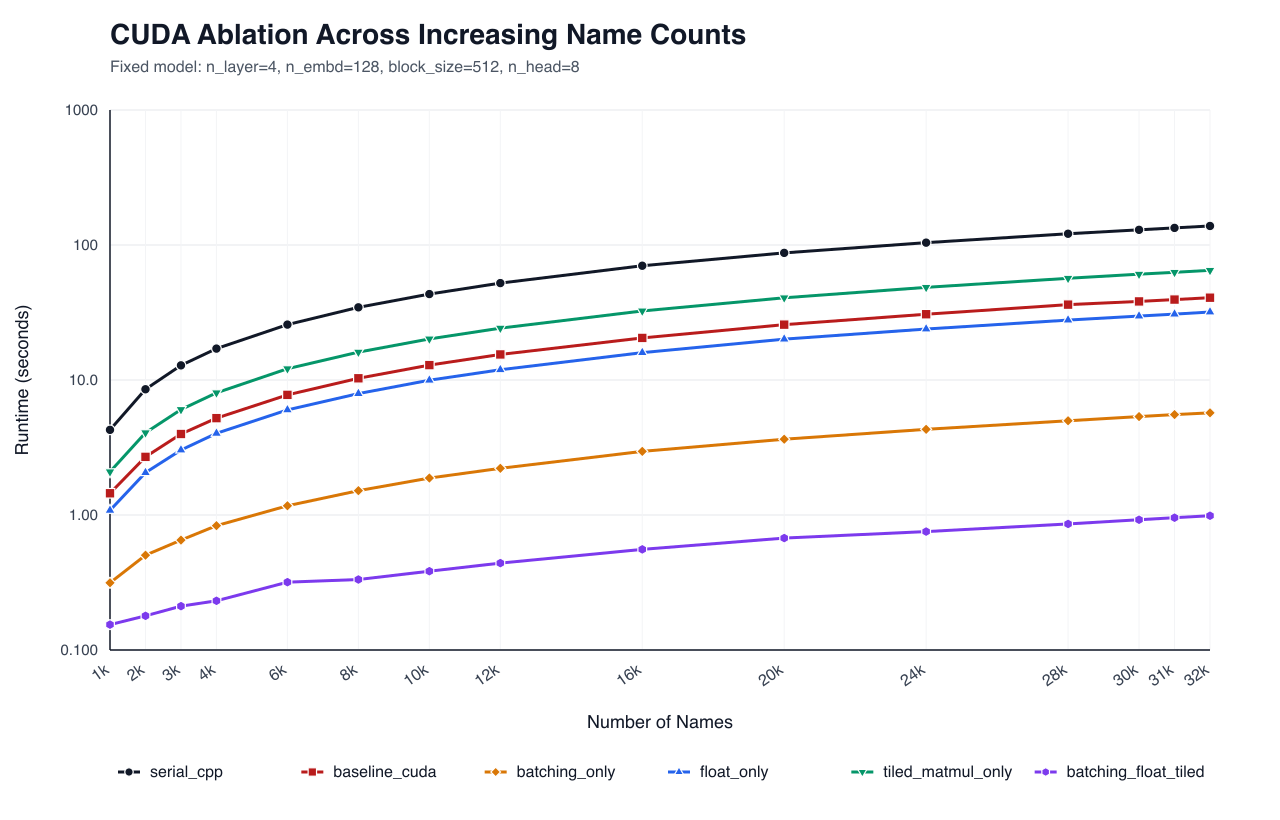
\includegraphics[width=\linewidth]{cuda_ablation_names.png}
    \caption{Ablation Study of Implemented Optimizations}
    \label{result:ablation}
\end{figure}

Our profiling results for the optimized implementation can be found in \strongappref{appendix:profile}.


\section{Conclusion}

In this project, we successfully transitioned the GPT-2 forward pass from a sequential Python implementation to a 
high-performance, parallelized CUDA C++ application. By identifying and addressing the bottlenecks 
inherent in serial execution, we demonstrated the immense computational advantages of GPUs for transformer-based 
architectures.

Our final implementation leverages several important parallel computing techniques: batched processing of sequences, tiled 
matrix multiplication, and a transition from double-precision to single-precision floating point accuracy. The 
results show the effectiveness of these strategies, achieving a speedup of over 10,000$\times$ compared to the serial Python 
baseline and over 500$\times$ compared to the serial C++ implementation on large-scale model configurations. Notably, our 
CUDA implementation outperformed the PyTorch implementation in several benchmarks, especially in smaller 
to mid-sized workloads where Python overhead is more pronounced.

However, our performance analysis also revealed that while our CUDA implementation is very powerful, its scaling 
behavior for extremely large datasets and model sizes slightly lags behind that of industry-standard frameworks like 
PyTorch. This suggests that further optimizations, such as more sophisticated memory coalescing, reducing 
global memory traffic between operations, and the use of specialized hardware features like Tensor Cores, would be 
necessary to maintain a performance advantage given larger models.

Future work could extend this project by implementing the backward pass to support full model training, reducing memory 
usage by further reducing floating point precision, and exploring multi-GPU parallelism. Ultimately, this project serves 
as a clear demonstration of how parallel computing principles are the driving forces behind the modern era of 
large language models.
\section{Link to Source and other resources}

The full project source, including the implementations, benchmark scripts, and generated results, is available at \href{https://github.com/sigggy/CUDA-parallel-gpt}{\textcolor{blue}{\nolinkurl{https://github.com/sigggy/CUDA-parallel-gpt}}}.

\section{Feedback}

\todoadd{Add any class feedback or suggestions requested by the template.}


\clearpage
\appendix
\onecolumn

\section{Benchmark Presets}
\label{appendix:presets}

\begin{table}[h]
\centering
\setlength{\tabcolsep}{4pt}
\renewcommand{\arraystretch}{1.05}
\resizebox{0.65\textwidth}{!}{%
\begin{tabular}{@{}lccccc@{}}
\hline
\textbf{Preset} & \textbf{n\_layer} & \textbf{n\_embd} & \textbf{block\_size} & \textbf{n\_head} & \textbf{steps} \\
\hline

\hline
S  & 1 & 64  & 128 & 4  & 2000  \\
M  & 2 & 128 & 128 & 8  & 5000  \\
L  & 4 & 256 & 256 & 8  & 10000 \\
VL & 6 & 384 & 512 & 12 & 20000 \\
XL & 8 & 512 & 512 & 16 & 30000 \\

\hline
MS5          & 1 & 64  & 512 & 4  & 5000 \\
MM5          & 2 & 128 & 512 & 8  & 5000 \\
ML5          & 4 & 256 & 512 & 8  & 5000 \\
MVL5         & 6 & 384 & 512 & 12 & 5000 \\
MXL5         & 8 & 512 & 512 & 16 & 5000 \\

\hline
\end{tabular}%
}
\caption{Model Configurations Used in Experiments}
\label{tab:benchmark_presets}
\end{table}

\section{Serial Implementation Prompt}
\label{appendix:serial-prompt}
The initial serial C++ baseline discussed in Section~2 was generated from the prompt ``Convert the provided microGPT-style Python implementation into a clean serial C++ program,'' with the following requirements:
\begin{itemize}[noitemsep, topsep=0pt]
    \item Keep the model architecture equivalent to the Python version, including token embeddings, positional embeddings, stacked transformer blocks, RMSNorm, causal self-attention, MLP feedforward layers, residual connections, and final logits with cross-entropy loss.
    \item Implement only the forward pass.
    \item Do not use CUDA, OpenMP, Eigen, BLAS, or any external numerical library.
    \item Use simple C++ data structures such as \texttt{std::vector} over \texttt{double} values and explicit loops.
    \item Process one input sequence at a time.
    \item Preserve the same tensor shapes and operation ordering as the Python version.
    \item Include clear helper functions for embedding lookup, RMSNorm, linear projection, attention score computation, softmax, MLP projection, ReLU, residual addition, and logits/loss computation.
    \item Prioritize readability and correctness over optimization.
    \item Use deterministic parameter loading from fixture files so the C++ implementation can be checked against the Python baseline.
    \item Organize the code so later versions can reuse the same structure for batching and CUDA parallelization.
\end{itemize}

\section{Optimized Profiling Results}
\label{appendix:profile}
\begin{table}[h]
\centering
\setlength{\tabcolsep}{4pt}
\renewcommand{\arraystretch}{1.05}
\resizebox{0.65\textwidth}{!}{%
\begin{tabular}{@{}lccccc@{}}
\hline
\textbf{Kernel} & \textbf{Time (\%)} & \textbf{Total Time} & \textbf{Calls} & \textbf{Avg} & \textbf{Max} \\
\hline
linear\_kernel & 85.88\% & 2.40485 s & 1372 & 1.7528 ms & 6.9377 ms \\
rmsnorm\_kernel & 4.52\% & 126.59 ms & 476 & 265.95 $\mu$s & 424.22 $\mu$s \\
self\_attn\_kernel & 4.45\% & 124.61 ms & 224 & 556.29 $\mu$s & 1.1746 ms \\
cross\_entropy\_loss\_kernel & 3.73\% & 104.36 ms & 28 & 3.7271 ms & 6.7604 ms \\
relu\_kernel & 0.58\% & 16.380 ms & 224 & 73.123 $\mu$s & 133.66 $\mu$s \\
add\_vec\_kernel & 0.42\% & 11.762 ms & 448 & 26.254 $\mu$s & 50.016 $\mu$s \\
embedding\_lookup\_kernel & 0.02\% & 481.57 $\mu$s & 28 & 17.198 $\mu$s & 31.776 $\mu$s \\
\hline
\end{tabular}%
}
\label{tab:profile_optimization}
\caption{CUDA Kernel Profiling Results for the Optimized Parallel Implementation}
\end{table}


\clearpage
\bibliographystyle{ACM-Reference-Format}
\bibliography{references}

\end{document}
